\documentclass[border=10mm]{standalone}
\usepackage{tikz}
\usetikzlibrary{arrows, shapes.gates.logic.US, shapes.gates.logic.IEC, calc}

\tikzset{
    my-and-gate/.style={
        and gate US, draw, rotate=0, logic gate inputs=nn
    },
}

\begin{document}

\resizebox{10cm}{!}{

    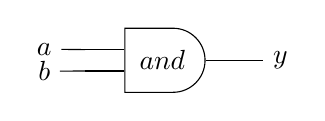
\begin{tikzpicture}[label distance=2mm]

        % INPUTS
        \node[] (A)    at (0,.28)  {\normalsize $a$};
        \node[] (B)    at (0,0)    {\normalsize $b$};

        % OUTPUTS
        \node[] (Y)    at (3,.14)  {\normalsize $y$};
        
        % AND, WIRES AND CONNECTOR POINTS
        \node[my-and-gate]  (AND)    at ($(B) + (1.5, .14)$)         {\normalsize $and$};
        \coordinate[]       (ANDIN1) at ($(AND.input 1) + (-.5, 0)$) {};
        \coordinate[]       (ANDIN2) at ($(AND.input 2) + (-.5, 0)$) {};
        \coordinate[]       (ANDOUT) at ($(AND.output)  + (.5, 0)$)  {};
        \draw (AND.input 1) -- (ANDIN1);
        \draw (AND.input 2) -- (ANDIN2);
        \draw (AND.output)  -- (ANDOUT);

        % INPUT CONNECTIONS
        \draw (A) -- (ANDIN1);
        \draw (B) -- (ANDIN2);
        
        % OUTPUT CONNECTIONS
        \draw (ANDOUT) -- (Y);

    \end{tikzpicture}
}

\end{document} 
